\section{L'Internet des Objets}

L'Internet des objets, abrégé en IoT, ou Cyber Physical Systems est un réseau non pas composé d'ordinateurs ou de serveurs mais de nombreux composants bien plus petits par leurs tailles et limités par leurs caractéristiques.

Ce nouveau type de réseau apporte de nouvelles contraintes pour le développement de logiciel en particulier.

Ces contraintes vont de la limitation de la puissance de calcul, du stockage limité, de la durée de vie de la batterie et jusqu'à la complexité de gestion d'un réseau distribué.

\section{L'environnement Contiki}

Les limites physiques des nœuds composant les réseaux étudiés font qu'un système d'exploitation spécifique doit être utilisé en lieu et place du classique GNU/Linux.

Les nœuds principalement utilisés pour les expériences sont des M3, globalement les nœuds sont sur une architecture ARM, le processeur est cadencé à 72MHz, possède 64kB de RAM et 16MB de ROM.

Ces nœuds sont également équipés de différents capteurs tels que:
\begin{itemize}
\item un capteur de luminosité,
\item un thermomètre,
\item un baromètre,
\item un accéléromètre/magnétomètre,
\item un gyromètre
\end{itemize}

\begin{figure}[ht!]
\centering
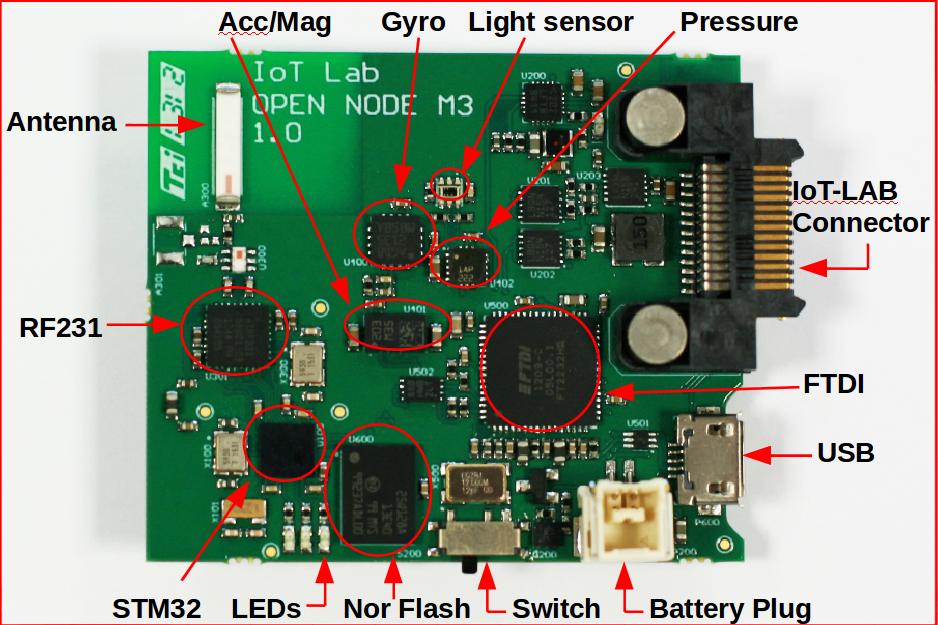
\includegraphics[width=90mm]{images/m3opennode.png}
\caption{Vue détaillée d'un nœud M3}
\end{figure}

Ces capteurs sont la source des données extérieures et la raison de déployer des CPS.

\subsection{Réseau de nœuds}

Les réseaux de capteurs ne sont généralement pas mis en réseau comme des ordinateurs classiques, où chaque nœud du réseau peut accéder directement à internet.

Ici le réseau est de type \emph{mesh}, c'est à dire qu'un nœud est connecté à internet, on l'appelle le \emph{border router}, et que les autres sont ou reliés au \emph{border router} ou à un autre nœud indirectement connecté au \emph{border router}.

%schéma d'un réseau mesh

De cette manière pour récupérer du contenu sur internet un nœud peut avoir besoin d'effectuer plusieurs bonds. Également la connexion entre nœuds n'est pas filière mais par ondes radio, réduire au maximum les communications entre nœuds est donc un enjeu de gain de temps puisque les débits de communication sont très faible et de batterie puisque qu'une communication peut impacter tout un réseau dans certains structures.

\subsection{Principales différences}

De par ces différences le développement logiciel est radicalement différent de ce que l'on peut trouver lorsque l'on cible un ordinateur «classique».

Dans notre cas ces limites sont dues au langage de développement, le langage C, qui n'est pas compilé pour utiliser la \emph{libc} standard, non disponible sur l'environnement \emph{Contiki}. Cette restriction, entre autre, empêche l'utilisation de générateur de code.

Bien que possible sur un environnement \emph{Contiki} l'allocation dynamique de mémoire ne doit pas se faire en utilisant le classique \emph{malloc}. En effet ce dernier gère mal la fragmentation de la mémoire. Pour palier à cela \emph{Contiki} met à disposition des développeurs d'autres méthodes telles que \emph{memb} et \emph{mmem}.\footnote{https://github.com/contiki-os/contiki/wiki/Memory-allocation}

Pour rester proportionné à l'espace disque et à la puissance de calcul des nœuds \emph{Contiki} utilise en système de fichiers spécifique nommé \emph{Coffee} qui est une  implémentation du \emph{Contiki File System}\footnote{https://github.com/contiki-os/contiki/wiki/File-systems}, CFS. Ce dernier empêche l'utilisation des fonctions habituelles de gestion d'accès disque telle que \emph{fopen}.


\section{Testbed FIT IoT-lab}

FIT est un projet financé par divers organismes de l'enseignement supérieurs et de la recherche afin de mettre à disposition des entreprises et des chercheurs des structures pour les aider dans leurs travaux.

IoT-lab\footnote{https://www.iot-lab.info/} est une infrastructure permettant l'accès à différents sites en France hébergeant du matériel dédié à l'Internet des Objets.

FIT permet l'accès à plus de 2700 nœuds répartis sur 7 différents testbed tel qu'à Rennes, Grenoble ou Rocquencourt. Les testbeds proposent jusqu'à 3 architectures différentes, dont des \emph{m3}.

%citer cette page en annexe https://www.iot-lab.info/deployment/

La réservation de nœuds se fait directement sur le site web. L'utilisateur a libre choix sur le site, le nombre et le type de nœud. Dans la limite des ressources disponibles et pour une durée conseillée d'au maximum 2 heures.

Une fois des nœuds réservés et obtenus il est possible d'y déployer un nouveau firmware. Toutes ces opérations, de la réservation de nœuds au flashage d'un nouveau firmware, sont directement réalisable en ligne de commande\footnote{https://www.iot-lab.info/tutorials/experiment-cli-client/}.

\section{model@runtime, Kevoree et KMF}

\subsection{model@runtime}

Le développement de réseaux distribués de machines de plus en plus complexes a amené la volonté et le besoin de pouvoir les reconfigurer plus aisément. L'intérêt peut être de mettre à jour un module fonctionnant sur une machine tout en minimisant le temps durant lequel le module ne sera pas fonctionnel.

Pour cela le paradigme du \emph{model@runtime} utilise un modèle servant à définir l'architecture détaillée d'un réseau à un instant \emph{t}.
 
%citer le papier de François en biblio

\subsection{KMF}

\emph{KMF}, Kevoree Modeling Framework\footnote{http://kevoree.org/kmf/}, est un langage de modeling s'inspirant de \emph{EMF}, Eclipse Modeling Framework\footnote{http://www.eclipse.org/modeling/emf/}, mais conçut pour répondre aux besoins du \emph{model@runtime}.

L'objectif de \emph{KMF} est de, à partir d'un méta-modèle, produire une structure de données et des outils de manipulation.

\subsection{Kevoree}

\emph{Kevoree} est un projet open-source implémentant le paradigme du \emph{model@runtime}. Les versions principales sont écrites en \emph{Java} et en \emph{Javascript} mais des implémentations en \emph{C} et \emph{C++} ont également été implémentées. Chaque version de \emph{Kevoree} est basée sur une version de \emph{KMF}. 

\emph{Kevoree} offre des mécanismes de comparaison et de fusion de modèles pour permettre l'adaptation de systèmes distribués.

\subsubsection{Kevoree-c}

La version utilisée durant ce stage est \emph{kevoree-c}\footnote{https://github.com/kYc0o/kevoree-c-reloaded} réalisée par Francisco Javier Acosta Padilla dans le cadre de sa thèse. Contrairement aux autres versions de \emph{Kevoree} celle-ci n'a pas été obtenue par génération depuis un méta-modèle mais a été écrite à la main.


%les différentes versions
%Chargement de binaire, ELF loader1
%surtout faire la transition sur le besoin de produire une implémentation depuis un modèle de Kevoree écrit en KMF